\documentclass[11pt,a4paper]{article}

\usepackage[T1]{fontenc}
\usepackage[utf8]{inputenc}
\usepackage{lmodern}
\usepackage{microtype}
\usepackage{amsmath}
\usepackage{amssymb}
\usepackage[margin=2.6cm]{geometry}
\usepackage{booktabs}
\usepackage{tabularx}
\usepackage{array}
\usepackage{graphicx}
\usepackage{caption}
\usepackage{float}
\usepackage{xcolor}
\usepackage{listings}
\usepackage{fancyhdr}
\usepackage[hidelinks]{hyperref}

\definecolor{accent}{HTML}{275CB2}
\definecolor{notebg}{HTML}{F1F5FB}
\definecolor{warnbg}{HTML}{FBF2EA}
\definecolor{rule}{HTML}{C6D0E0}
\definecolor{code}{HTML}{2A3242}
\definecolor{comment}{HTML}{6B7688}

\hypersetup{colorlinks=true, linkcolor=accent, urlcolor=accent}

\captionsetup{font=small, labelfont={bf,color=accent}, width=0.92\textwidth}

\pagestyle{fancy}
\fancyhf{}
\renewcommand{\headrulewidth}{0.4pt}
\fancyhead[L]{\footnotesize\sffamily Human-Centric AI --- Implementation Report}
\fancyhead[R]{\footnotesize\sffamily Kartik Anand, 676049}
\fancyfoot[C]{\footnotesize\thepage}

\setlength{\parskip}{0.55em}
\setlength{\parindent}{0pt}

\renewcommand{\arraystretch}{1.15}
\setlength{\emergencystretch}{2.5em}

% Section headings in the accent colour, sans serif. Done by hand because
% sectsty and titlesec are both absent from this TeX installation.
\makeatletter
\renewcommand\section{\@startsection{section}{1}{\z@}%
  {-3.5ex \@plus -1ex \@minus -.2ex}{2.2ex \@plus.2ex}%
  {\normalfont\Large\sffamily\bfseries\color{accent}}}
\renewcommand\subsection{\@startsection{subsection}{2}{\z@}%
  {-3.0ex \@plus -1ex \@minus -.2ex}{1.4ex \@plus .2ex}%
  {\normalfont\large\sffamily\bfseries\color{accent}}}
\renewcommand\paragraph{\@startsection{paragraph}{4}{\z@}%
  {2.4ex \@plus1ex \@minus.2ex}{-0.8em}%
  {\normalfont\normalsize\sffamily\bfseries\color{code}}}
\makeatother

% Callout boxes, built by hand: tcolorbox and mdframed are not in this TeX install.
\newsavebox{\calloutbuf}
\newenvironment{callout}[1][notebg]
  {\par\medskip\begin{lrbox}{\calloutbuf}%
   \begin{minipage}{\dimexpr\linewidth-24pt\relax}\setlength{\parskip}{0.4em}}
  {\end{minipage}\end{lrbox}%
   \noindent\colorbox{notebg}{\hspace{4pt}\usebox{\calloutbuf}\hspace{4pt}}\par\medskip}

\newenvironment{warncallout}
  {\par\medskip\begin{lrbox}{\calloutbuf}%
   \begin{minipage}{\dimexpr\linewidth-24pt\relax}\setlength{\parskip}{0.4em}}
  {\end{minipage}\end{lrbox}%
   \noindent\colorbox{warnbg}{\hspace{4pt}\usebox{\calloutbuf}\hspace{4pt}}\par\medskip}

\lstset{
  language=Python,
  basicstyle=\ttfamily\footnotesize\color{code},
  commentstyle=\itshape\color{comment},
  keywordstyle=\color{accent},
  stringstyle=\color{comment},
  showstringspaces=false,
  breaklines=true,
  frame=leftline,
  framesep=8pt,
  rulecolor=\color{rule},
  xleftmargin=10pt,
  aboveskip=1em,
  belowskip=1em,
}

\newcommand{\file}[1]{\texttt{\small #1}}

\title{\vspace{-1.4cm}\sffamily\color{accent}\bfseries
       Human-Centric Artificial Intelligence\\[0.25em]
       \Large\mdseries Implementation Report}
\author{Kartik Anand \quad---\quad Matriculation 676049\\[0.3em]
        \small Hamburg University of Technology \quad SoSe 2026}
\date{\small \today}

\begin{document}
\maketitle
\thispagestyle{fancy}

\begin{callout}
This report records how the coursework was built and, more importantly, why each
open decision was settled the way it was. The course briefs leave several choices
deliberately unspecified; those are the passages worth reading. Project~1 is
complete and described in full. Projects~2 to~4 have their own sections, filled in
as the work is done.
\end{callout}

\tableofcontents

\vspace{1em}

% ============================================================================
\section{Scope, layout and environment}

\subsection{Repository}

All four projects live as separate Django apps inside one Django project, as the
brief requires, and the whole thing is submitted as a git repository. The working
tree sits at \file{\textasciitilde/Documents/TUHH/SoSe2026/HCAI/}:

\begin{center}
\begin{tabularx}{0.94\textwidth}{@{}lX@{}}
\toprule
\textbf{Path} & \textbf{Contents} \\
\midrule
\file{HCAI-PBL/}   & The Django repository. Fork of \file{ppaamm/HCAI-PBL}; remote is \file{k-styles/HCAI-PBL}. \\
\file{docs/}       & Course overview and the project briefs. \\
\file{lectures/}   & The twelve lecture PDFs and the demo notebooks. \\
\file{data/}       & \file{iris.csv} and \file{diabetes.csv}, used during development. \\
\file{report/}     & The source of this document. \\
\file{.venv/}      & Python environment. \\
\bottomrule
\end{tabularx}
\end{center}

Inside the Django repository, \file{home/} is the landing page, \file{demos/} is
the course's example app left untouched, \file{pbl/} holds the settings and root
URL configuration, and each project gets its own app directory.

\subsection{Environment and running it}

Python 3.13 with Django 6.1, scikit-learn 1.9, pandas 3.0, matplotlib 3.11; the
exact versions are pinned in \file{requirements.txt}. From the repository root:

\begin{lstlisting}[language=bash, keywordstyle=\color{code}]
python -m venv .venv
source .venv/bin/activate
pip install -r requirements.txt
python manage.py migrate
python manage.py runserver
\end{lstlisting}

The site is then at \url{http://127.0.0.1:8000/home/}.

\subsection{Status of the four projects}

\begin{center}
\begin{tabularx}{0.94\textwidth}{@{}llX@{}}
\toprule
\textbf{Project} & \textbf{Status} & \textbf{Subject} \\
\midrule
1 & Complete   & Automated machine learning: a supervised learning interface. \\
2 & Complete   & Explainability: model complexity, counterfactuals, feature effects. \\
3 & Complete   & Active learning for learning-to-defer, with its own PDF report. \\
4 & Complete   & Preference elicitation: a movie recommender, a designed user study, and its own PDF report. \\
\bottomrule
\end{tabularx}
\end{center}

% ============================================================================
\section{Project 1 --- Automated Machine Learning}

\subsection{What the brief asks}

Four tasks. Task~1: put the group members on the home page, from Python rather
than from the template. Task~2: create the \file{project1} app and link it from
the home page. Task~3: a module that uploads a CSV, reads it and visualises it.
Task~4: implement the full training pipeline, and --- the part that carries the
marks --- decide \emph{what the user should be in control of and what should be
done automatically}.

That last question is not decoration. Lecture~1 works through a ridge regression
on the diabetes dataset, chooses the penalty, reports the error, and closes the
slide with ``Conclusion: no human needed!'' --- immediately followed by a slide
titled ``Bringing the human back in the loop'', which lists the choices that were
silently made by a person at every step: who collected the data, who picked the
model, who picked the evaluation criterion, who will use the result. The project
is named \emph{Automated Machine Learning} for the same reason. The application
was therefore built so that the division of labour between the user and the
machine is the thing you see first, not an implementation detail.

\subsection{Structure of the app}

\begin{center}
\begin{tabularx}{0.94\textwidth}{@{}lX@{}}
\toprule
\textbf{File} & \textbf{Responsibility} \\
\midrule
\file{data.py}     & Reading a CSV, discarding bookkeeping columns, deciding classification vs.\ regression. \\
\file{learning.py} & Model and score registries, the train/test split, fold construction, the sweep, the selection rule. \\
\file{plots.py}    & Matplotlib figures written into \file{MEDIA\_ROOT}. \\
\file{models.py}   & \texttt{TrainingRun}: one row per sweep, so runs can be compared afterwards. \\
\file{forms.py}    & Upload and training forms; the training form's choices depend on the problem type. \\
\file{views.py}    & Three pages --- data, visualisation, training --- plus the run log. \\
\bottomrule
\end{tabularx}
\end{center}

Roughly 1780 lines including templates and stylesheet. The uploaded file is
written to \file{MEDIA\_ROOT} under a random token and only the token is kept in
the session; the rows are re-read on each request. Keeping a parsed
\texttt{DataFrame} in the session would serialise the entire dataset on every
request, and files of this size cost nothing to re-read.

\subsection{Reading the data}

The brief fixes the format --- header in the first row, target in the last column
--- and then leaves three things open. Each was settled as an explicit rule.

\paragraph{Discarding an index column.} The brief says datasets sometimes carry a
per-row id and that one ``can either assume that the provided datasets do not
include such a column, or filter it out''. Matching on the column name is the
obvious approach and it is wrong: \file{patient\_id} can be a genuine feature. The
rule used here is structural --- integer, unique across every row, and
consecutive. A column satisfying all three is numbering the rows and nothing else.

\begin{lstlisting}
def looks_like_row_number(col):
    if not pd.api.types.is_integer_dtype(col):
        return False
    v = np.sort(col.to_numpy())
    if len(np.unique(v)) != len(v) or len(v) < 10:
        return False
    return bool((np.diff(v) == 1).all())
\end{lstlisting}

\paragraph{Classification or regression.} The brief asks explicitly whether the
user must state the problem type or whether the app should detect it. The answer
taken here is \emph{both}: detect it, show the verdict on screen, and let the
user overrule it.

The overrule is a single click on the visualisation page, not a second upload.
The file is already on disk and the problem type is only a note in the session,
so requiring the same file to be uploaded again in order to change one setting
would be ceremony rather than a safeguard --- and it would discard the plots and
the position the user had reached. Where the override is impossible the request
is refused, the reason is given, and the dataset they had stays exactly as it
was. A non-numeric target is labels. A numeric target is labels
only if its values are whole numbers and there are few enough distinct ones to
plausibly be classes. The common shortcut --- a fixed cutoff of ten distinct
values --- misreads a twelve-class problem in one direction and a twenty-row
regression table in the other, so the cutoff grows with the size of the data:
\[
  \text{cutoff} \;=\; \min\!\bigl(20,\ \max(10,\ \lfloor\sqrt{N}\rfloor)\bigr).
\]
For the 150 rows of iris this gives 12; its three species fall well inside it.

\paragraph{Columns and rows that cannot be used.} Non-numeric feature columns are
dropped, as are rows with a missing target or missing features. Nothing is
imputed silently. Every such action is reported on the page as a note, naming the
column and the row count, because a cleaning step the user cannot see is a
cleaning step the user cannot check.

\subsection{Visualisation}

The brief sets a floor --- upload, read, visualise --- and then says plainly that
the more is done here, the higher the mark. The module was built to that, not to
the floor. Everything is matplotlib written into the media directory and loaded
as an image, which is the route the course's \file{demos} app demonstrates.

Two defects in that demo were not copied. Its figure filename is a fixed
\file{myplot.png}, so two browser tabs overwrite each other's plots; here the
filename is keyed to the session token. And it never sets the \texttt{Agg}
backend, which fails in a server thread; that is set before \texttt{pyplot} is
imported.

\paragraph{What was read.} Before any figure, the first ten rows are shown as the
application understands them, after the dropped columns. If a file has been
misparsed, every plot below it is answering the wrong question, and the user
should be able to see that in one glance rather than infer it from a strange
histogram.

\paragraph{The scatter the brief names.} Two shapes are described: for
classification, two chosen features coloured by class; for regression, either two
features or \emph{one feature against the target label}. Both are supported. The
axes are chosen by the user, and on a regression problem the target itself
appears in the axis list, at which point colour is dropped because it would only
repeat an axis. Plotting a feature straight against the outcome is the plainest
view of the thing being predicted, so it is the default there.

\paragraph{Every pair at once.} A single scatter answers whether two chosen
features separate the target. It cannot answer which two should have been chosen.
A pair grid --- every combination as a scatter, each feature's own histogram on
the diagonal --- answers that in one figure (Figure~\ref{fig:iris-pairs}). On a
wide table this would be unreadable, so it is capped at six columns, chosen by
the ranking below and named on the page.

\paragraph{Which features carry the answer.} The features are ranked by how much
each says about the target on its own. For regression this is the magnitude of
the correlation. For classification it is the ratio of between-class to
within-class variance --- the quantity a one-way ANOVA is built on: a feature
scores highly when the class means are far apart relative to the scatter inside
each class.
\[
  F \;=\; \frac{\sum_c n_c (\bar{x}_c - \bar{x})^2 \,/\, (k-1)}
                {\sum_c (n_c - 1)\, s_c^2 \,/\, (N-k)}
\]
On iris this puts petal length and petal width an order of magnitude above the
sepal measurements, which is the same conclusion the histograms reach visually.
Both measures look at one feature at a time, so neither can see two features that
are useless alone and decisive together; the page says so rather than letting the
ranking be read as a feature selector.

\paragraph{All features at once.} The columns are standardised and projected onto
the two directions of greatest variance (Figure~\ref{fig:iris-pca}). This is
written out as an SVD of the centred matrix rather than imported, since that is
all principal components are. It answers a question none of the other figures
can: if the classes separate here but in no single pair above, the information is
spread across features rather than sitting in one, which is an argument for a
model that combines them. On iris the leading component carries 73.0\,\% of the
variance and the second 22.9\,\%, matching the published values for this dataset
and serving as a check on the implementation.

\paragraph{The rest.} Per-feature histograms split by class show where the classes
overlap --- on iris the petal measurements separate them and the sepal
measurements do not (Figure~\ref{fig:iris-dist}). On a regression problem the
target gets a panel of its own, because a skewed outcome is worth knowing about
before choosing a score: squared error will chase the tail. A correlation heatmap
shows which features carry the same information twice, which is exactly what the
penalty term in ridge regression exists to handle. Finally a descriptive
statistics table, and for classification a class-balance table showing the
proportions that the test split and every fold preserve.

\begin{figure}[H]
\centering
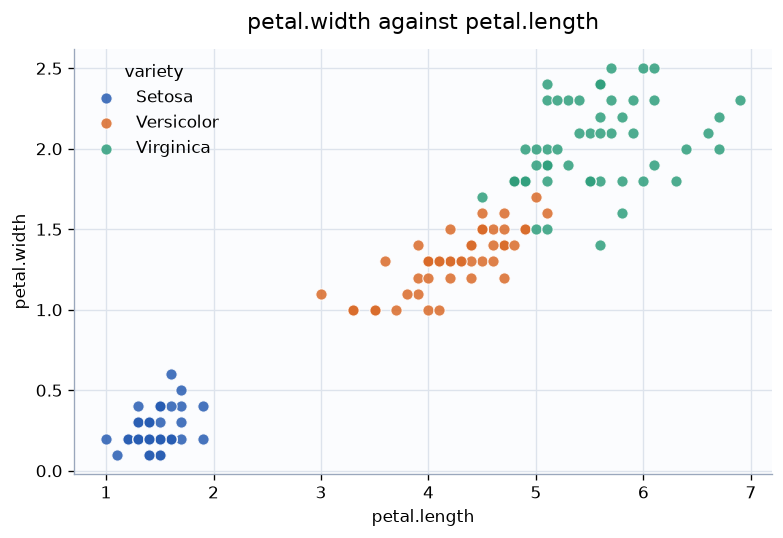
\includegraphics[width=0.78\textwidth]{figures/iris-scatter.png}
\caption{Petal length against petal width on the iris data, coloured by species.
Setosa is linearly separable from the other two on these axes; Versicolor and
Virginica touch. Choosing the sepal measurements instead gives a far muddier
picture --- which is the point of letting the user choose the axes.}
\label{fig:iris-scatter}
\end{figure}

\begin{figure}[H]
\centering
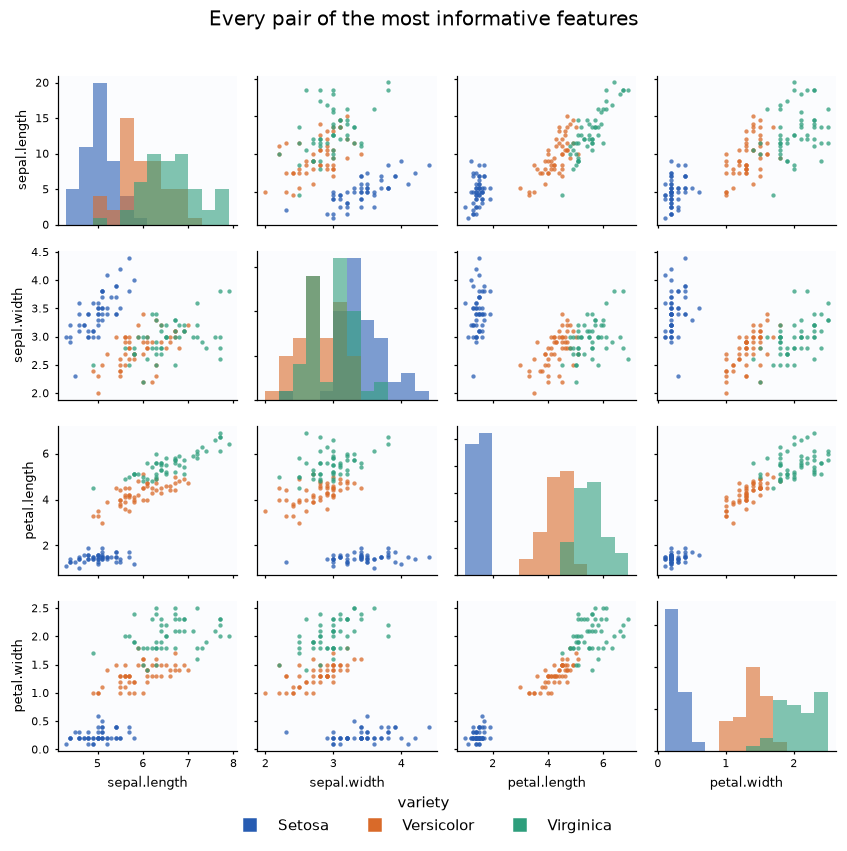
\includegraphics[width=0.80\textwidth]{figures/iris-pairs.png}
\caption{Every pair of features at once, with each feature's own distribution on
the diagonal. Read in one pass: Setosa detaches from the other two in any panel
involving a petal measurement, and Versicolor and Virginica touch everywhere.
That is the whole modelling problem, before a model has been fitted.}
\label{fig:iris-pairs}
\end{figure}

\begin{figure}[H]
\centering
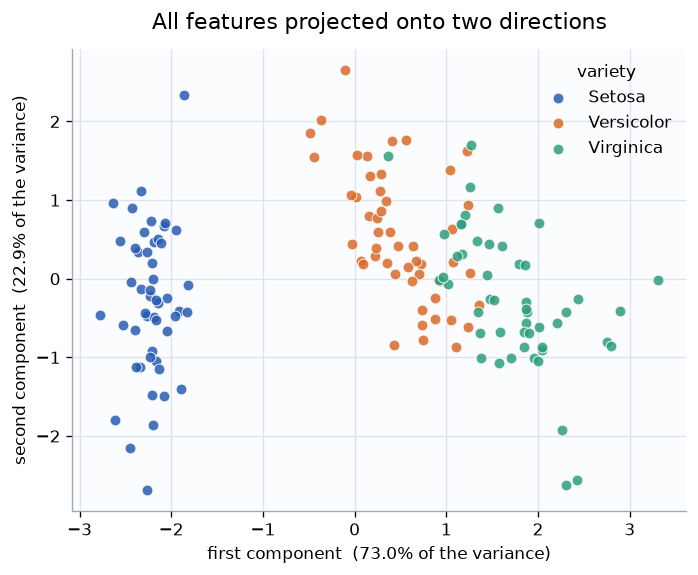
\includegraphics[width=0.62\textwidth]{figures/iris-pca.png}
\caption{All four features standardised and projected onto their two directions
of greatest variance, computed as an SVD of the centred matrix. The leading
component carries 73.0\,\% of the variance, the second 22.9\,\% --- the published
figures for standardised iris, which makes this a check on the implementation as
well as a plot.}
\label{fig:iris-pca}
\end{figure}

\begin{figure}[H]
\centering
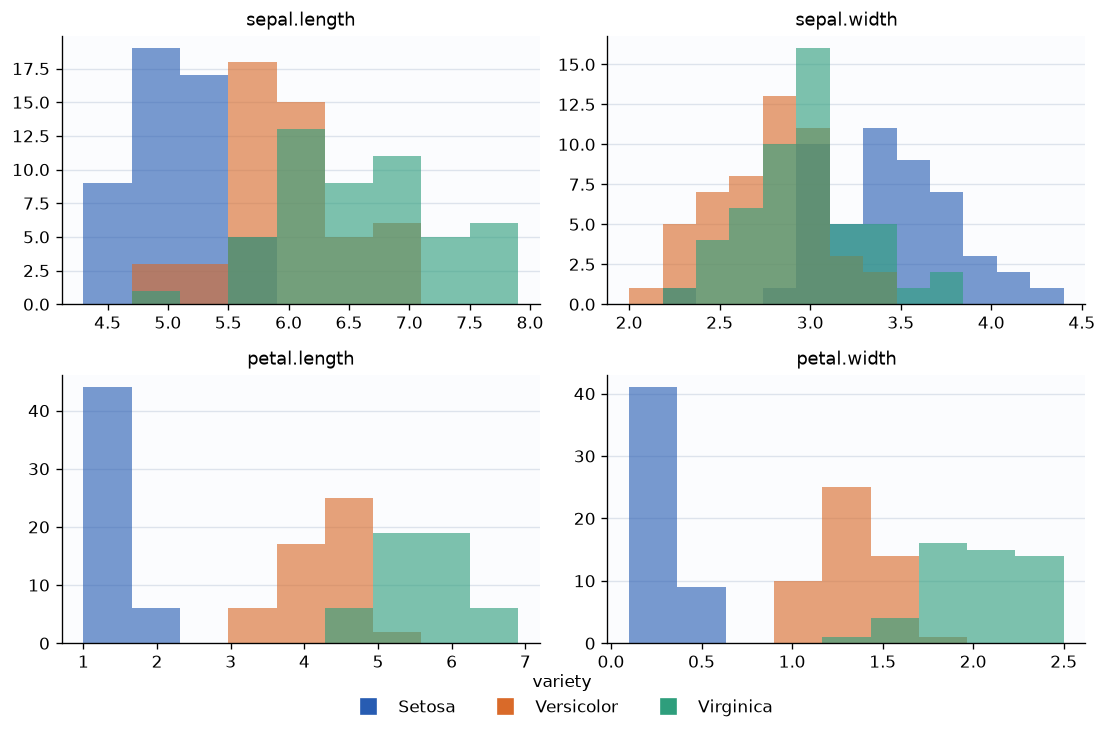
\includegraphics[width=0.86\textwidth]{figures/iris-dist.png}
\caption{Per-feature distributions split by species. The two petal features
separate the classes almost completely on their own; the two sepal features
overlap heavily. A user who reads this before training knows what to expect from
the model.}
\label{fig:iris-dist}
\end{figure}

\subsection{Model selection}

This is the part of the project with genuine design content, and the part where
the obvious library call is the wrong answer. \texttt{GridSearchCV} would do the
whole of Task~4 in one line. It would also make every decision the brief is
asking about, invisibly. The pipeline below is written out instead.

\paragraph{Holding out a test set.} The rows are split before anything else
happens. For classification the split is taken class by class and every class is
forced to contribute at least one test row, so a rare class cannot disappear from
the evaluation entirely.

\paragraph{Constructing folds.} The training rows are dealt into $k$ folds by
shuffling the indices of each class separately and distributing them round-robin.
Every fold then carries close to the class proportions of the whole training set.
This matters on small data: with iris and five folds, an unstratified shuffle can
hand one fold twice as many of a species as another, and the resulting validation
curve is partly measuring the shuffle rather than the model.

\begin{lstlisting}
def make_folds(y, n_folds, rng, stratify):
    idx = np.arange(len(y))
    groups = [idx[y == label] for label in np.unique(y)] if stratify else [idx]

    folds = [[] for _ in range(n_folds)]
    for group in groups:
        for offset, position in enumerate(rng.permutation(group)):
            folds[offset % n_folds].append(position)
    return [np.array(sorted(f)) for f in folds]
\end{lstlisting}

Checked on iris with a 25\,\% test split: 114 training rows dealt into folds of
24, 24, 24, 21 and 21, each holding exactly equal numbers of the three species,
and the folds verified to be disjoint and to cover every training row.

\paragraph{The sweep.} For each candidate value of the hyperparameter, the model
is fitted $k$ times, once per fold, and scored on the held-out fold. The mean, the
standard error across folds, and --- separately --- the score on the rows each
model was fitted on are all recorded. The last of these is not needed to pick a
winner; it is recorded because the gap between the two curves is what overfitting
looks like, and the user should be able to see it rather than be told about it.

\paragraph{Choosing a value: the one-standard-error rule.} Taking the best mean is
taking the maximum of $k$ noisy numbers. The default rule here instead collects
every value whose cross-validated score lies within one standard error of the
best, and among those keeps the \emph{simpler} model --- the shallower tree, the
larger neighbourhood, the stronger penalty. Those values are not distinguishable
from the winner given the spread of the folds, so preferring the plainer one costs
almost nothing on this sample and is less likely to be an artefact of one
particular shuffle. There is no scikit-learn equivalent for this. The user can
switch back to plain argmax from the form; both rules are offered because which
one is right is a judgement, not a fact.

\begin{lstlisting}
peak = (max if score.higher_is_better else min)(rows, key=lambda r: r.mean)

if score.higher_is_better:
    tied = [r for r in rows if r.mean >= peak.mean - peak.se]
else:
    tied = [r for r in rows if r.mean <= peak.mean + peak.se]

if rule == "one_se":
    order = (lambda r: r.value) if algo.simpler == "low" else (lambda r: -r.value)
    winner = min(tied, key=order)
else:
    winner = peak
\end{lstlisting}

\paragraph{Keeping the test score honest.} The hyperparameter is chosen entirely
inside the training rows. The test rows are used once, after the choice is fixed,
for a single final fit and evaluation. Lecture~1's demonstration selects the
penalty on the test set and then quotes that same test error as the result; the
number that comes out of that procedure has already been optimised against. The
distinction is small on the diabetes data and large in principle, and it is
stated on the training page so the user knows which of the two they are reading.

\subsection{Models, hyperparameters and scores}

One hyperparameter is swept per model, which is what the brief describes. Models
whose behaviour depends on distances or on a coefficient norm are wrapped in a
standardising pipeline; trees are not, because they are invariant to feature
scale.

\begin{center}
\begin{tabularx}{0.94\textwidth}{@{}llX@{}}
\toprule
\textbf{Model} & \textbf{Swept} & \textbf{Simpler end} \\
\midrule
\multicolumn{3}{@{}l}{\itshape Classification} \\
$k$-nearest neighbours & $k$ & larger $k$ --- a smoother boundary \\
Decision tree          & max depth & shallower \\
Logistic regression    & $C$ & smaller $C$ --- a stronger penalty \\
SVM, RBF kernel        & $C$ & smaller $C$ \\
\addlinespace
\multicolumn{3}{@{}l}{\itshape Regression} \\
Ridge regression       & $\alpha$ & larger $\alpha$ \\
$k$-nearest neighbours & $k$ & larger $k$ \\
Decision tree          & max depth & shallower \\
\bottomrule
\end{tabularx}
\end{center}

Ridge with a swept $\alpha$ is lecture~1's own worked example, kept deliberately
so the application can be checked against a known result. Scores are accuracy and
macro F1 for classification, and $R^2$, mean squared error and mean absolute
error for regression. All of them are reported after every run; the one selected
in the form only decides the winner. Reporting a single number would reproduce
precisely the habit lecture~1 criticises --- the defect-detection example, where a
false negative and a false positive are not remotely the same event.

\subsection{Explaining the vocabulary in place}

Lecture~1 states the problem this section solves: ``In practice, most users are
no machine learning experts: they ignore the characteristics of the algorithms
and models, and they have no understanding nor intuition on the parameters.''
An interface that offers a box labelled $C$ and no way to find out what $C$ is
has handed the user a choice they are not equipped to make, and then presented
the result as though they had made it.

Thirty-three terms are written out in plain language --- every model, every
hyperparameter, every score, and the ideas behind them: overfitting, standard
error, cross-validation, the held-out test set, the selection rule. Each has its
own page. No formula appears without first being said in words, and each page
ends with what to actually do.

The delivery matters more than the content. A glossary the user has to navigate
to is help that arrives after the confusion has already cost them something, so
the links are placed where the words are:

\begin{itemize}
\item \textbf{Inline, in the prose.} The sentence describing the split of
responsibility reads ``\emph{Yours}: the model, the values to try, how much data
is held back, how many folds, the score, and how ties are broken'' --- and each
of those six phrases is itself a link, marked with a dotted underline. Hovering
shows the one-line answer without leaving the page at all. There are 36 such
links on the training page and 20 on the visualisation page.

\item \textbf{Beside form labels.} A small outlined marker next to each field.
Three of them are rewritten by script as the dropdowns change: select a decision
tree and the marker beside ``values to try'' points at the page on tree depth;
select $k$-nearest neighbours and it points at the page on $k$; change the score
and its marker follows.
\end{itemize}

\subsection{What each candidate got wrong, on request}

The confusion matrix for the winning model answers ``where was it wrong''. It
cannot answer the more useful question, which is how the mistakes \emph{changed}
as the hyperparameter moved.

Every row of the sweep table can therefore be expanded to show its own error
breakdown. The predictions come from the cross-validation that has already
happened: each fold's model predicts the fold held out from it, and those
out-of-fold predictions are collected per candidate. They cost nothing extra to
compute, and no candidate is ever scored on rows it was fitted on --- so this is
available for every value without spending the test set on any of them. For
regression, where no confusion matrix exists, the same panel reports the typical
miss, the worst miss, and whether the model leans high or low.

The panels are collapsed by default. Nine extra tables opened on arrival would
bury the result; the question only arises once the user has a reason to ask it.

The iris sweep shows why it is worth asking. A tree of depth~1 scores 0.6667,
which merely says ``poor''. Expanding it says what poor means here: Setosa 38 of
38, Versicolor 38 of 38, Virginica \emph{0 of 38}. The one-question tree never
predicts the third species at all. That is a different and far more actionable
fact than a single number, and it is invisible in the score column.

\subsection{Answering Task 4: who decides what}

\begin{center}
\begin{tabularx}{0.94\textwidth}{@{}XX@{}}
\toprule
\textbf{The user decides} & \textbf{The app does} \\
\midrule
The model & Builds class-balanced folds \\
The values to sweep & Fits every candidate \\
The size of the test set & Keeps the test rows out of the selection \\
The number of folds & Reports every applicable score, not just one \\
The score to select on & Skips values that cannot be fitted, and says which \\
How ties are broken & Records the run in the log \\
The random seed & \\
\bottomrule
\end{tabularx}
\end{center}

The split is deliberate. Everything on the left is a judgement that depends on
what the user is trying to achieve; everything on the right is mechanical, and
automating it removes drudgery rather than authority.

Next to the form sits a second button, \emph{Decide for me}, which runs every
model for the detected problem type over its default grid and keeps the winner,
asking nothing at all. It then shows what it decided --- including the models it
discarded and their scores --- with a note saying that a model further down the
table may be easier to explain or cheaper to run, for a difference in score too
small to be worth the trade. On the iris data the automatic route selects
$k$-nearest neighbours with $k=13$ and reaches 0.9167 test accuracy, while a
decision tree of depth~3, chosen manually, reaches 0.9444 and can be read off in
three questions. That contrast is the argument of lecture~1 rendered as two
buttons on one page.

Every run --- manual or automatic --- is written to a \texttt{TrainingRun} row and
listed at \file{/project1/history/}, so two sets of settings can be compared after
the fact instead of from memory. This is the use of Django models the brief
suggests for projects that offer several learning algorithms.

\subsection{Results}

\paragraph{Iris, decision tree, accuracy.} Table~\ref{tab:iris} is the case the
selection rule exists for. Nine depths were swept; depths 3 through 14 are
\emph{identical} in cross-validation while the training score climbs to a perfect
1.000. Plain argmax has nothing to separate them. The one-standard-error rule
keeps depth~3, which reaches 0.9444 accuracy and 0.9441 macro F1 on the 36
held-out rows, and which a person can actually read.

\begin{table}[H]
\centering
\small
\begin{tabular}{@{}rrrrl@{}}
\toprule
\textbf{Max depth} & \textbf{CV accuracy} & \textbf{$\pm$ SE} & \textbf{On training rows} & \\
\midrule
1  & 0.6667 & 0.0000 & 0.6667 & \\
2  & 0.9476 & 0.0170 & 0.9759 & \\
3  & 0.9655 & 0.0158 & 0.9847 & \textbf{kept} \\
4  & 0.9655 & 0.0158 & 0.9956 & tied \\
5  & 0.9655 & 0.0158 & 0.9978 & tied \\
6  & 0.9655 & 0.0158 & 1.0000 & tied \\
8  & 0.9655 & 0.0158 & 1.0000 & tied \\
10 & 0.9655 & 0.0158 & 1.0000 & tied \\
14 & 0.9655 & 0.0158 & 1.0000 & tied \\
\bottomrule
\end{tabular}
\caption{Five-fold sweep over tree depth on iris, 114 training rows. Everything
from depth~3 onwards is the same model as far as cross-validation can tell; the
only thing that changes is how much of the training set it has memorised.}
\label{tab:iris}
\end{table}

\begin{figure}[H]
\centering
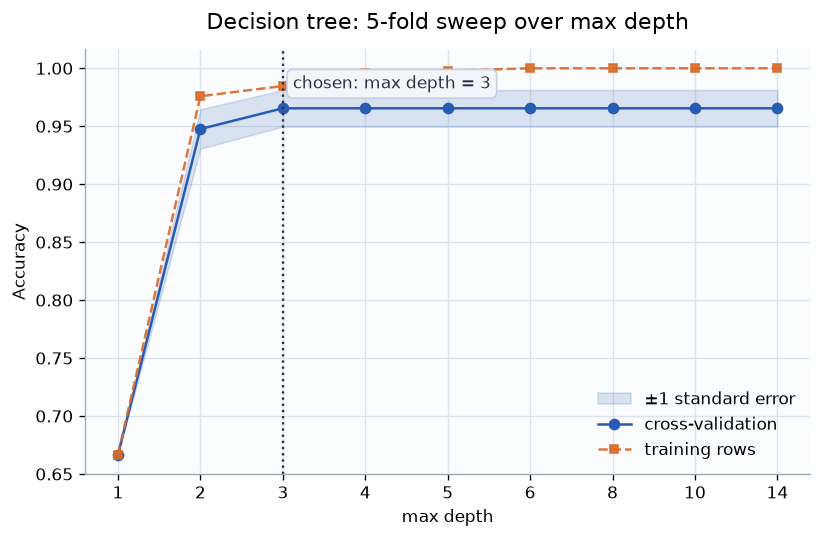
\includegraphics[width=0.82\textwidth]{figures/iris-sweep.png}
\caption{The same sweep as a curve. The solid line is cross-validation with its
one-standard-error band; the dashed line is the score on the rows each model was
fitted on. Where the two separate, the model is memorising rather than learning.}
\label{fig:iris-sweep}
\end{figure}

\paragraph{Diabetes, ridge regression, mean squared error.} Here the rule
actually overrules the peak. The best mean sits at $\alpha=1$, but $\alpha=100$
lies within one standard error of it, and the far more strongly penalised model is
kept. On the held-out rows it scores marginally \emph{better} --- 2889.2 against
2893.8 --- which is luck rather than proof, but it is not the trade going wrong.

\begin{table}[H]
\centering
\small
\begin{tabular}{@{}rrrrl@{}}
\toprule
$\boldsymbol{\alpha}$ & \textbf{CV MSE} & \textbf{$\pm$ SE} & \textbf{On training rows} & \\
\midrule
0.001 & 3026.80 & 183.48 & 2840.24 & tied \\
0.01  & 3026.73 & 183.56 & 2840.24 & tied \\
0.1   & 3026.12 & 184.26 & 2840.29 & tied \\
1     & 3024.18 & 188.70 & 2842.79 & best mean \\
10    & 3024.72 & 194.38 & 2861.22 & tied \\
100   & 3082.98 & 198.44 & 2981.10 & \textbf{kept} \\
1000  & 4150.11 & 167.53 & 4107.01 & \\
\bottomrule
\end{tabular}
\caption{Five-fold sweep over the ridge penalty on the diabetes data. The final
test MSE of 2889.2 sits alongside lecture~1's reported 2856 for the same dataset
and model --- close enough to treat the pipeline as validated against a known
result, and different enough to be explained by the split and by the fact that the
lecture selects its penalty on the test set.}
\label{tab:diabetes}
\end{table}

\begin{figure}[H]
\centering
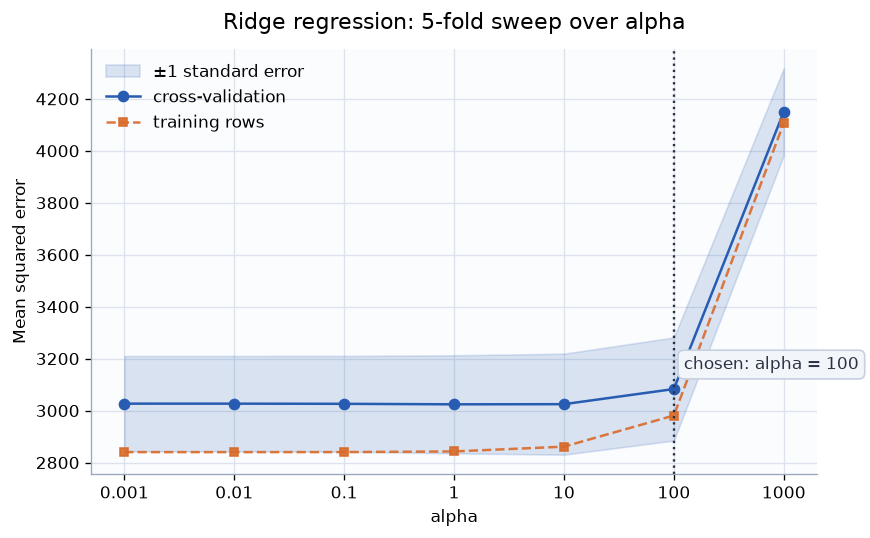
\includegraphics[width=0.82\textwidth]{figures/diabetes-sweep.png}
\caption{Ridge on the diabetes data, scored by $R^2$. The curve is almost flat
across four orders of magnitude of $\alpha$ before it collapses --- which is the
honest shape of this problem, and is invisible if a grid search returns only its
argmax.}
\label{fig:diabetes-sweep}
\end{figure}

\subsection{Verification}

A script exercises every view through Django's test client: both datasets, all
seven model and rule combinations, custom grids, the automatic route, the run log,
and ten error paths. Thirty-four checks, no failures, no server errors and no
browser console errors. The generated figures were inspected directly rather than
assumed, and the two-dimensional projection was checked against the published
variance shares for standardised iris.

Four defects were found this way and fixed:

\begin{enumerate}
\item A three-row file reported ``no usable numeric features'' instead of ``too
few rows'', because the index-column filter consumed its only feature column
first. The row-count guard now runs before any column is discarded, and the filter
requires at least ten rows before it will call a column bookkeeping.

\item On a small dataset the default $k$-nearest-neighbours grid contained values
of $k$ larger than the number of rows a fold could train on, and scikit-learn
raised. Candidates that cannot be fitted are now filtered out before the sweep and
named on the page, rather than aborting the run.

\item The warning shown after an automatic run asserted that ``a decision tree of
depth~3 would have been almost as good'' --- true for iris and false in general.
It was replaced with text that points at the leaderboard instead of hardcoding a
result.

\item Forcing the problem type to regression on a dataset whose target is text
returned a server error, because nothing checked that the override was possible
before the feature ranking tried to correlate against the string
\texttt{Setosa}. The override is refused at load time now, with a message naming
the column and what to do instead.
\end{enumerate}

The fourth is the instructive one. The override had been tested before release
--- but only on a numeric target, which is the one case where forcing regression
happens to work. A test that exercises a feature on the single input it was
written against confirms nothing. The problem type is now checked across every
combination of the three settings and three shapes of target column: text,
continuous, and small whole numbers where either reading is defensible. The
opposite direction, forcing a continuous target into classes, was found to be
technically caught already but to report itself by listing two hundred singleton
``classes''; it now says that the column reads as a quantity and suggests
regression.

\subsection{Where the inputs are}

\begin{center}
\begin{tabularx}{0.94\textwidth}{@{}lX@{}}
\toprule
\textbf{Location} & \textbf{What to change} \\
\midrule
\file{home/views.py}, \texttt{GROUP} & Names and matriculation numbers. Set in Python, as Task~1 requires. \\
The upload form at \file{/project1/} & The dataset, and the problem type if the detected one is wrong. \\
\file{project1/learning.py}, \texttt{ALGORITHMS} & Default hyperparameter grids, if the form's per-run field is not enough. \\
\bottomrule
\end{tabularx}
\end{center}


% ============================================================================
\section{Project 2 --- Explainability}

Palmer Penguins: 344 rows, of which 333 are complete. Four numeric measurements
(bill length, bill depth, flipper length, body mass) and three categorical
columns (island, sex, year) predict the species. That split between numeric and
categorical is what Tasks 4 and 5 turn on.

One stratified split of 233 training and 100 test rows is made once and shared by
every model on the page. Task 2 compares models by test accuracy, so a model must
not be able to look better merely by having been handed an easier test set.

\subsection{Tasks 1 to 3: complexity as something the user holds}

Equation (1) of the brief trades empirical loss against a complexity measure
$\Omega$. Task 2 makes that trade interactive: a slider on $\lambda$ selects
whichever trained model maximises $\mathrm{acc}_{\text{test}} - \lambda\,\Omega(f)$.

\paragraph{Reading the tree back out.} Task 1 asks for the tree to be shown.
\texttt{plot\_tree} is the conventional answer and is included, but it is also the
first thing to stop being readable --- past a dozen leaves it is a wall of small
boxes. Since the subject of this project is precisely whether a person can follow
the model, the fitted tree is also walked directly and rendered as one sentence
per root-to-leaf path. At $\lambda = 0.02$ the whole model is three lines:

\begin{center}
\small
\begin{tabularx}{0.94\textwidth}{@{}Xr@{}}
\toprule
\textbf{Rule} & \textbf{Support} \\
\midrule
flipper $\le 207.5$ and bill length $\le 43.35$ $\;\to\;$ Adelie & 100 penguins, 98\,\% pure \\
flipper $> 207.5$ $\;\to\;$ Gentoo & 87 penguins, 94\,\% pure \\
flipper $\le 207.5$ and bill length $> 43.35$ $\;\to\;$ Chinstrap & 46 penguins, 93\,\% pure \\
\bottomrule
\end{tabularx}
\end{center}

One detail matters for readability. The model is fitted on one-hot columns, so a
split reads internally as \texttt{island=Biscoe} $\le 0.5$. Printing that would be
faithful to the arithmetic and useless to a reader, so categorical splits are put
back into words as ``island is not Biscoe''.

\paragraph{Choosing $\Omega$ for logistic regression (Task 3).} The brief fixes
$\Omega$ for a tree as the leaf count and leaves the linear case open. The measure
used here is \textbf{the number of original features carrying a non-zero
coefficient}, under an L1 penalty.

The reasoning is that $\Omega$ should measure the same thing in both cases: how
much of the model a person has to read before they can say what it does. For a
tree that is the number of questions it may ask. For a linear model it is the
number of features that must be looked up, and a coefficient of zero costs the
reader nothing. L1 is what makes the count move at all --- an L2 penalty shrinks
coefficients without ever reaching zero, which would leave $\Omega$ pinned at the
full feature count for every setting and make the slider inert. Original features
are counted rather than encoded columns: ``island'' is one thing to go and find
out, whether it expands into two dummy columns or ten. Task 4 referring to the
slider as ``sparsity'' points the same way.

\paragraph{Which models the slider can actually reach.} For a fixed candidate,
$\mathrm{acc} - \lambda\Omega$ is a straight line in $\lambda$ with slope
$-\Omega$. Maximising over candidates is therefore taking the upper envelope of a
family of lines, and only candidates whose line touches that envelope are ever
selected. Plotted as $(\Omega, \mathrm{acc})$, that envelope is the upper concave
hull: anything strictly below it loses at every $\lambda$ to something simpler,
something more accurate, or a blend of the two.

This is worth computing rather than leaving implicit, because it converts the
slider from a dial to be dragged blindly into a short list with exact
boundaries. Of the ten distinct trees trained, \emph{four} can ever be selected;
the 5-, 6-, 7-, 8-, 10- and 13-leaf trees are unreachable at every $\lambda$ even
though they look perfectly reasonable in the results table.

\begin{table}[H]
\centering
\small
\begin{tabular}{@{}llrrl@{}}
\toprule
$\boldsymbol{\lambda}$ \textbf{from} & \textbf{up to} & $\boldsymbol{\Omega}$ & \textbf{accuracy} & \\
\midrule
0.000 & 0.005 & 12 & 0.980 & most accurate available \\
0.005 & 0.010 & 4  & 0.940 & \\
0.010 & 0.140 & 3  & 0.930 & the three-rule tree above \\
0.140 & --    & 2  & 0.790 & one question, two answers \\
\bottomrule
\end{tabular}
\caption{Every model the tree slider can produce, and the exact range of
$\lambda$ that produces it. The widest band by far is the three-leaf tree, which
is also the one a person can read.}
\label{tab:p2-bands}
\end{table}

\begin{figure}[H]
\centering
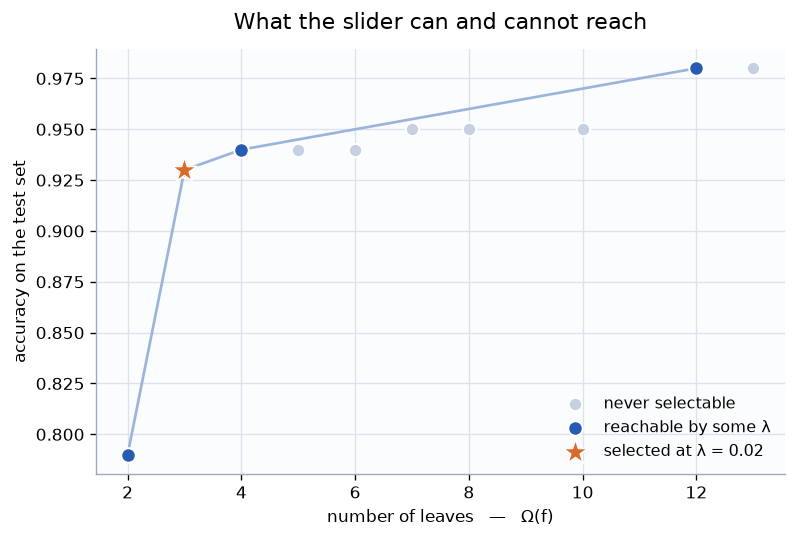
\includegraphics[width=0.80\textwidth]{figures/p2-frontier.png}
\caption{Accuracy against complexity for the ten trees. Filled points are on the
upper concave hull and are reachable; grey points are dominated and no setting of
the slider produces them.}
\label{fig:p2-frontier}
\end{figure}

\begin{figure}[H]
\centering
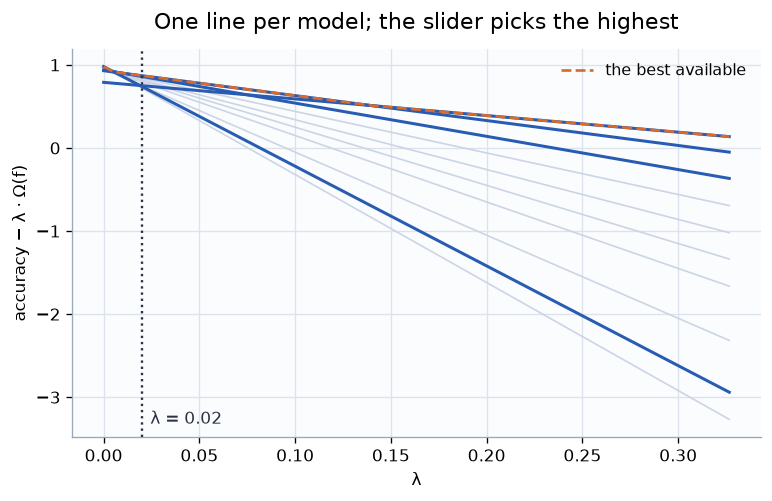
\includegraphics[width=0.80\textwidth]{figures/p2-objective.png}
\caption{The same thing as lines. Each model is $\mathrm{acc} - \lambda\Omega$;
the slider picks whichever is highest at the chosen $\lambda$. The greyed lines
spend their whole lives underneath someone else's, which is what ``unreachable''
means.}
\label{fig:p2-objective}
\end{figure}

The logistic family behaves differently and instructively: every one of its five
distinct models is on the hull, so the slider genuinely sweeps from all seven
features at 0.99 accuracy down to a model using none at all and scoring 0.44 ---
which is the majority-class rate, exactly as it should be.

\subsection{Task 4: counterfactual explanations}

The brief's recipe is followed directly --- sample around $x$, keep the draws the
model assigns to the desired class, rank by MAD-weighted $L^1$ distance, show the
closest few --- with three decisions that the brief hands over.

\paragraph{Noising categorical data.} The brief asks the question explicitly.
Numeric features get Gaussian noise with standard deviation
$\text{spread} \times \mathrm{MAD}(\text{feature})$, so one spread setting means
the same thing to body mass in grams and bill depth in millimetres, and it is the
same scale the ranking distance uses. Categorical features cannot be nudged ---
there is nothing between Biscoe and Dream --- so each is left alone with
probability $1 - \text{flip}$ and otherwise redrawn from the values actually
observed. Drawing from the empirical distribution rather than uniformly keeps
rare combinations rare, so a proposal no penguin would ever be does not get
ranked highly.

\paragraph{Distance across mixed types.} A categorical change counts 1 and no
change counts 0, which puts it on the same order as a typical numeric change once
the numerics are divided by their own MAD.

\paragraph{Sparsity, which turned out to matter most.} Perturbing all four
measurements on every draw means every counterfactual returned has all four
changed, and ``alter everything slightly'' is close to useless as advice. Each
draw therefore first picks how many numeric features it may touch --- uniformly
from one to all four --- and leaves the rest exactly as they were. Sparse
proposals then exist to be found, and since changing fewer features costs less
distance they win the ranking whenever they work at all.

The effect is large. Before this change, the closest counterfactual for penguin
\#0 towards Chinstrap altered all four measurements at distance 1.79. After it,
the answer is a single change --- bill length from 39.1 to 43.6\,mm, distance
0.96 --- which is an explanation someone can act on.

If nothing is found the search widens over four rounds, growing the number of
draws and the noise. Reaching Gentoo from an Adelie needs the second round and
returns a longer answer: grow the flippers past 207\,mm \emph{and} be on Biscoe.
Both are biologically real distinctions in this dataset, which is a reassuring
sign that the search is finding structure rather than noise.

\subsection{Task 5: PDP and ALE, written from scratch}

The brief requires these to be implemented rather than imported. They are
computed from the fitted model's predicted probabilities and numpy arithmetic:
there is no \texttt{sklearn.inspection}, no \texttt{partial\_dependence}, and no
ALE package anywhere in the file.

\paragraph{PDP.} For each grid value $v$, every row in the data has the feature
forced to $v$, the model is asked, and the answers are averaged:
\[
  \mathrm{PDP}_c(v) \;=\; \frac{1}{n}\sum_{i=1}^{n} P\!\left(c \,\middle|\, x_i \text{ with } x_{ij} := v\right).
\]
Grid points are placed by quantile so they follow the data rather than the axis.

\paragraph{ALE.} Following the lecture's definition, with the integral estimated
per bin and the curve centred to zero mean over the data. The expectation is
conditional --- inside each bin only rows whose own value falls in that bin
contribute --- which is the entire advantage over the PDP. On this dataset
flipper length and body mass move together, so forcing a flipper to 230\,mm while
leaving body mass alone asks the model about an animal that does not exist. The
PDP averages over those; the ALE never constructs them.

\paragraph{Exact or discretised (the brief's question).} \emph{Logistic
regression admits exact derivatives.} The scores are linear in the standardised
inputs, so $\partial s_c / \partial x_j = W_{cj}/\sigma_j$, and pushing that
through the softmax gives
\[
  \frac{\partial p_c}{\partial x_j} \;=\; p_c\!\left(\frac{W_{cj}}{\sigma_j}
    - \sum_{c'} p_{c'}\frac{W_{c'j}}{\sigma_j}\right),
\]
which is written down in closed form and integrated across each bin. A class
gains probability only in so far as its own score rises faster than the
probability-weighted average, which is why one species' ALE curve must fall when
another's rises.

\emph{A decision tree does not.} It is piecewise constant: its derivative is zero
almost everywhere and undefined exactly on the split points, so there is nothing
to evaluate pointwise and finite differences across bin edges are forced. Both
paths are implemented and the interface states which one produced the curve on
screen.

That the two agree is the check that makes the derivative trustworthy. Computing
both ways for the logistic model on all four features, the curves match to
$1.5 \times 10^{-4}$ at worst --- a wrong derivative would diverge immediately.

\begin{figure}[H]
\centering
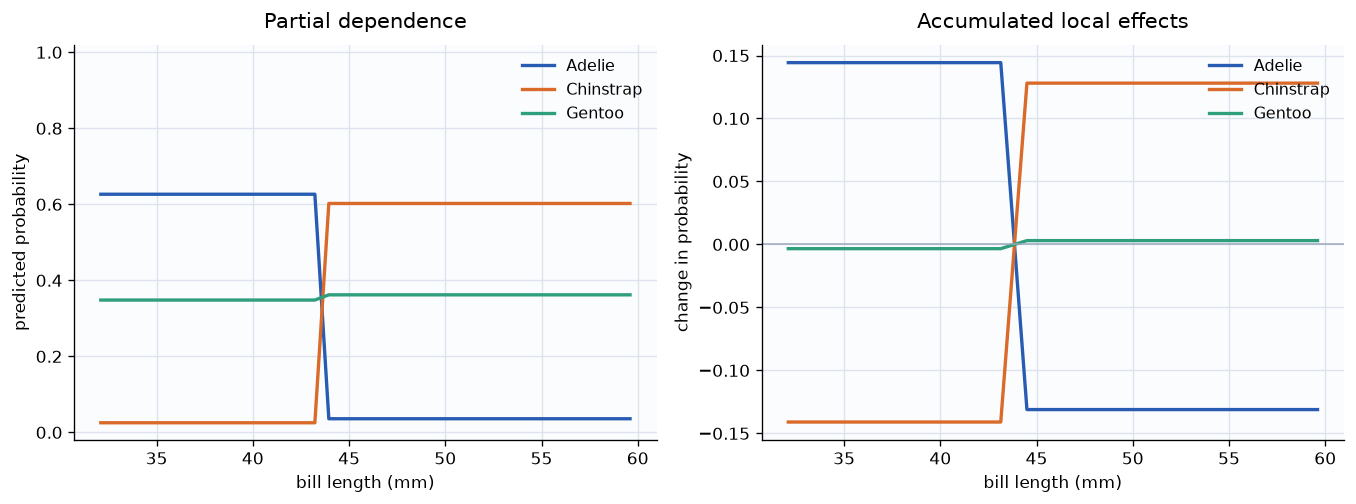
\includegraphics[width=0.94\textwidth]{figures/p2-effects-tree.png}
\caption{Bill length under the three-leaf tree. Both curves step at 43.35\,mm,
which is exactly the tree's split point --- the correct shape for a piecewise
constant model, and a useful sanity check on the implementation. Gentoo is flat
because this tree separates Gentoo on flipper length instead.}
\label{fig:p2-effects-tree}
\end{figure}

\begin{figure}[H]
\centering
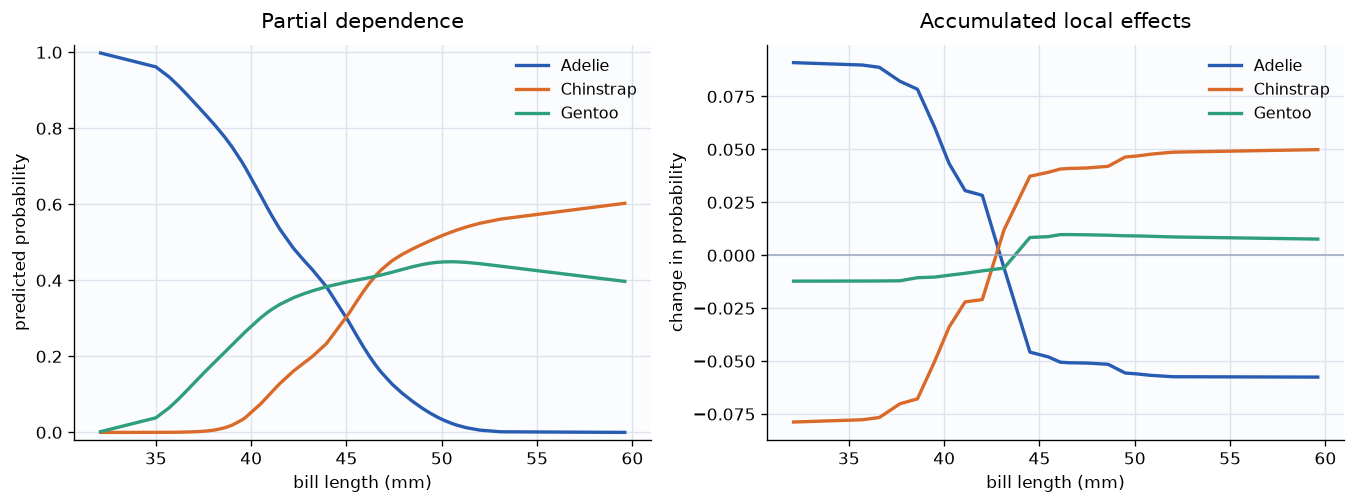
\includegraphics[width=0.94\textwidth]{figures/p2-effects-logistic.png}
\caption{The same feature under logistic regression, where the ALE integrand is
the closed-form softmax derivative. The transition is smooth rather than stepped,
as a differentiable model requires.}
\label{fig:p2-effects-logistic}
\end{figure}

\subsection{Keeping the regions linked}

The brief requires the counterfactual and feature-effect regions to be driven by
the model chosen in Tasks 1 to 3. The model class and $\lambda$ live in the
session and are set by one control strip that appears, identically, at the top of
all three regions. Switching from tree to logistic regression changes which
models the frontier offers, which model generates counterfactuals, and which
route the ALE takes --- all three were checked to move together.

\subsection{Verification}

A script drives every region through Django's test client: both model classes at
four values of $\lambda$, all three species as counterfactual targets from four
different penguins, all four features under both models, and the linkage between
regions. Every case passes. Alongside it:

\begin{itemize}
\item The hull was checked against brute force. Sweeping $\lambda$ over 35{,}000
values and taking the arg max directly reproduces exactly the set of models the
hull predicts, and the $\lambda$ bands agree with the arg max everywhere except
at a single floating-point tie on a boundary.

\item The PDP was checked against an independent hand computation at a chosen
grid point.

\item The two ALE routes were checked against each other, as described above.

\item Fixing the solver seed was necessary rather than cosmetic: \texttt{saga} is
stochastic, and without \texttt{random\_state} the fitted coefficients --- and so
$\Omega$, and so the whole frontier --- differed between runs. This was caught by
running the same computation in three separate processes and comparing.
\end{itemize}

\subsection{Marking what had to be our own}

The briefs single out particular components as things to implement or decide
ourselves. Rather than leave that as a claim, the requirements are held in one
registry (\file{home/own\_work.py}) which records the brief's exact words, the
file that satisfies each one, and what was done. Each such block in the code
carries a marker comment, and the page at \file{/home/own-work/} re-reads the
files and reports whether every marker is still present --- so deleting or moving
a marked block shows up as a failure rather than passing quietly. The relevant
entries are also shown in place, at the top of the region they govern.


% ============================================================================
\section{Project 3 --- Active Learning for Learning-to-Defer}

Complete, with its own 9-page PDF report at
\file{project3/report/project3-report.pdf}, downloadable from the project page as
the brief requires. The summary below states the brief; the report carries the
results and the argument.

The dataset is AG News: label news articles by topic. The system is allowed to
answer or to defer to a human expert, and the point of the project is to learn
\emph{when} deferring is worth it --- without being given the expert's labels up
front. Four required tasks and one optional one:

\begin{enumerate}
\item Train a classifier on the fully labelled training set and report test
accuracy. This is the baseline the human-AI team has to beat.

\item Design and implement at least one simulated expert. It must be imperfect
and, specifically, competent in particular regions of the input space rather than
uniformly noisy --- otherwise there is nothing for a deferral policy to learn.

\item Implement a learning-to-defer strategy, evaluated on the quality of the
deferral decisions and not only on accuracy.

\item Choose an active learning strategy for deciding which examples to show the
expert, given no expert labels at training time. Justify the choice.

\item (Optional) An interface where a person plays the expert.
\end{enumerate}

\subsection{Outcome}

A classifier right 92.3\,\% of the time is paired with a simulated expert right
69.9\,\% of the time; deciding per article which should answer raises the pair to
94.1\,\% while consulting the expert on 16\,\% of articles.

Two decisions carried the project. The simulated expert's competence is a function
of the input \emph{text}, not of the true label --- an expert reliable wherever the
label happens to be Sports could never be discovered by Task 4, because at query
time the label is exactly what is unknown. And every downstream target uses
out-of-fold predictions: the classifier makes 3{,}403 errors in-sample against
11{,}350 out-of-fold, so the in-sample figure would have understated failure by
3.3$\times$ and taught the deferral model that the classifier almost never needs
help.

A null result was found and kept. The second simulated expert shows no separation
between any query strategy, which narrows the claim from ``choosing questions
beats random'' to ``choosing questions helps when the expert's competence is
visible in the available features''.

% ============================================================================
\section{Project 4 --- Preference elicitation}

Complete, with its own 12-page PDF report at
\file{project4/report/project4-report.pdf} covering Tasks 1 to 3, downloadable
from the project landing page alongside the entry point to the study itself ---
the two-door arrangement the brief specifies.

The subject is a movie recommender that adapts quickly to a new user, built on the
IMDB 5000 Movie Dataset --- metadata for roughly 5000 films, with no user ratings.
A user's preferences are modelled by a utility $U(x) = w^{\mathsf{T}}x$, where $x$
is a feature vector for a film and $w$ is the user's latent preference vector to
be estimated from a small number of interactions.

\subsection{Task 1: the features, and the constraint that decides them}

The representation is 20-dimensional over a pool of 2{,}734 films (those with at
least 25{,}000 IMDB votes, since a participant comparing two films they have never
heard of is guessing from metadata rather than expressing a preference).

The argument is that the feature set is governed by the \emph{elicitation budget},
not by descriptive power. With $w$ fitted from roughly twenty-five responses, a
one-hot over the 2{,}398 directors is unidentifiable --- two random films share a
director well under once in a thousand times, so essentially every response
multiplies those weights by zero. A second rule excludes anything the participant
cannot see on the card: a feature that was invisible cannot have caused the
choice, but the fit will credit it anyway.

A genre earns a dimension only when two random films actually differ on it, which
happens with probability $2p(1-p)$; requiring one informative pair in ten puts the
cut at $p \geq 0.0528$ and admits fourteen genres. The threshold is computed in
\file{project4/data.py} rather than hardcoded, so the prose and the code cannot
drift apart.

\subsection{Task 2: Plackett--Luce}

A ranking is read as a sequence of choices --- favourite of ten, then of the
remaining nine --- each stage being Bradley--Terry widened past two alternatives.
The product of the stages is Plackett--Luce.

Three justifications, of which the middle one is the load-bearing one. It reduces
to Bradley--Terry exactly at $n = 2$. Its pairwise marginals \emph{are} the
Bradley--Terry probabilities, so both study arms estimate the same $w$ and can
legitimately be scored against a common held-out set --- without which the
comparison would be a category error. And the tempting alternative of splitting a
ranking into all 45 implied pairs is rejected on two grounds: it counts dependent
comparisons repeatedly, and it is not a distribution over the $n!$ orderings, so
it is not a likelihood at all.

\subsection{Task 3: the study, and a result that reversed it}

A 150-participant, between-subjects, time-matched, pre-registered design. Both
arms get the same eight-minute budget rather than the same number of tasks, since
what a recommender spends is the user's patience. Because $w$ is latent and no
distance to it is computable, the primary outcome is held-out prediction: an
identical block of ten fresh pairwise comparisons, scored by log loss.

The project began with the hypothesis that ranking wins, which is what the
per-task Fisher information says --- one ranking carries about 60$\times$ one
comparison. The power simulation written to size the study overturned it. Fixing
time rather than task count means eight minutes buys 80 comparisons or 5 rankings,
and the accumulated traces then come out at 118 against 129, a ratio of 1.09. And
the trace is the wrong summary: over a session the log-determinant is 17.6 nats
lower for ranking and its smallest eigenvalue 6.4$\times$ smaller, because 80
comparisons touch 160 films while 5 rankings touch 50, and the 45 comparisons
inside one ranking all lie in the span of that set's ten feature vectors. Ranking
piles up information about a few directions and leaves the rest to the prior.

Across 120 simulated participants per condition the arms tie when ranking is
assumed flawless ($d = 0.00$) and pairwise pulls clear as soon as later positions
get careless ($d = -0.34$ and $-0.51$). H1 was rewritten in the opposite
direction, which is what pre-registration exists to make visible.

\subsection{Task 4: the interface}

Consent and a stratification question, then blocked random assignment, then the
assigned design under a visible timer, then the held-out block, then a debrief
showing the participant their own fitted taste profile and five recommendations.

Responses go to database rows rather than the session, because session-only
storage loses everything when a tab closes. A pairwise choice is stored as a
ranking of length two, so the schema has one representation and the fitting code
never branches on the arm --- the practical payoff of Task 2's first
justification. Every draw derives from one stored seed per participant, so the
held-out block is fixed for them and cannot be rerolled by reloading.

Ranking supports drag-and-drop \emph{and} per-row arrow buttons, and the form
serves its hidden inputs in the presented order so that scripting-disabled
participants submit something coherent. This is not politeness: a drag-only
interface excludes participants invisibly, since they appear in the data as
abandonments and inflate exactly the secondary statistic being measured.

Twenty-four plain-language explanation pages are linked inline at the point each
term first appears, participant-facing screens included --- consent that requires
a statistics degree to understand is not informed consent.

% ============================================================================
\section{Use of AI tools}

The implementation was drafted with a large language model and then reviewed. The
repository contains \file{AI\_USAGE.md}, which records component by component what
that applies to. Both that file and this report are readable from inside the
application itself at \file{/project1/notes/} --- a convenience during
development, gated on \texttt{DEBUG} so the page and the file it serves both
return 404 in any other setting, and nothing has to be remembered and removed
before submission. In short: the Django wiring, the templates, the stylesheet and
the matplotlib figure code were drafted by the model; the three decisions in
Project~1 with more than one defensible answer --- the index-column rule, the
problem-type cutoff, and the fold construction with its selection rule --- were
settled against the brief and lecture~1 first, and the model was used to write
them down rather than to choose them. That distinction is the reason the project
does not simply call \texttt{GridSearchCV}, which is what a model asked to ``pick a
hyperparameter'' will reach for, and which is the answer the brief is designed to
get past.

\end{document}
